%%%% CAPÍTULO 4 - RESULTADOS E DISCUSSÃO

\chapter{Testes e Resultados}\label{cap:resultados}

Os testes foram feitos para prova de conceito e demonstração do funcionamento do protótipo, comparando as leituras obtidas \gls{CA} por este com as obtidas por um multímetro e por um osciloscópio.

O primeiro teste se diz respeito à leitura da tensão da rede local, sendo o sinal a ser lido as saídas de uma tomada de 127 V do laboratório. O \textit{setup} básico se encontra nas figuras \ref{fig:setup-main} e \ref{fig:setup-main2}. Para este teste se foi utilizado um reostato pois este tem uma grande capacidade de suportar correntes altas. A resistência deste se dá por 60,3 $\Omega$, como representado na \autoref{fig:resistencia-reostato-teste}.

Utilizando a lei de ohm $v = r \cdot  i$, espera-se uma leitura de corrente de 2.13 A.

\begin{figure}[htb!]
    \caption{\textit{Setup} básico para testes.}
    \label{fig:setup-main}
    \includegraphics[width=0.8\textwidth]{figuras/setup-basico.png}
    \fonte{}
\end{figure}

\begin{figure}[htb!]
    \caption{\textit{Setup} básico para testes completo.}
    \label{fig:setup-main2}
    \includegraphics[width=0.8\textwidth]{figuras/setup-basico-full.png}
    \fonte{}
\end{figure}

\begin{figure}[htb!]
    \caption{Resistência do reostato.}
    \label{fig:resistencia-reostato-teste}
    \includegraphics[width=0.3\textwidth]{figuras/resistencia-reostato-teste.png}
    \fonte{}
\end{figure}

A \autoref{fig:leitura-rede-osc} representa a leitura da tensão rede feita pelo osciloscópio, a \autoref{fig:leitura-rede-mult-t} representa a leitura de tensão feita pelo multímetro e a \autoref{fig:leitura-rede-mult-c} a leitura da corrente do circuito feita por este. Pelo protótipo, as figuras \ref{fig:leitura-rede-boy-ondas} e \ref{fig:leitura-rede-boy-valores}, respectivamente, representam as ondas e o valor destas leituras, além também da frequência.

\begin{figure}[htb!]
    \caption{Leitura da rede - Osciloscópio.}
    \label{fig:leitura-rede-osc}
    \includegraphics[width=0.8\textwidth]{figuras/leitura-rede-osc.png}
    \fonte{}
\end{figure}

\begin{figure}[htb!]
    \caption{Leitura da tensão da rede - Multímetro.}
    \label{fig:leitura-rede-mult-t}
    \includegraphics[width=0.3\textwidth]{figuras/leitura-rede-mult-t.png}
    \fonte{}
\end{figure}

\begin{figure}[htb!]
    \caption{Leitura da corrente do circuito - Multímetro.}
    \label{fig:leitura-rede-mult-c}
    \includegraphics[width=0.3\textwidth]{figuras/leitura-rede-mult-c.png}
    \fonte{}
\end{figure}

\begin{figure}[htb!]
    \caption{Leitura da rede e circuito pelo protótipo - Ondas}
    \label{fig:leitura-rede-boy-ondas}
    \includegraphics[width=0.8\textwidth]{figuras/leitura-rede-boy-ondas.png}
    \fonte{}
\end{figure}

\begin{figure}[htb!]
    \caption{Leitura da rede e circuito pelo protótipo - Valores}
    \label{fig:leitura-rede-boy-valores}
    \includegraphics[width=0.8\textwidth]{figuras/leitura-rede-boy-valores.png}
    \fonte{}
\end{figure}

Comparando os sinais obtidos, percebe-se que o protótipo propõe uma qualidade de leitura excepcional para este range, mantendo o formato da onda fiel e os valores com um erro dentro do proposto pelas especificações.

Além deste teste da leitura da rede, foram conduzidos dois outros testes para prova de conceito: leitura de um sinal de tensão de pico de aproximadamente 200 mVpp e a leitura de uma corrente na ordem de micro amperes.

O sinal de 200 mVpp foi gerado por um gerador de funções, conforme a \autoref{fig:ger-func-200}.

\begin{figure}[htb!]
    \caption{Gerador de funções - Sinal 200 mVpp.}
    \label{fig:ger-func-200}
    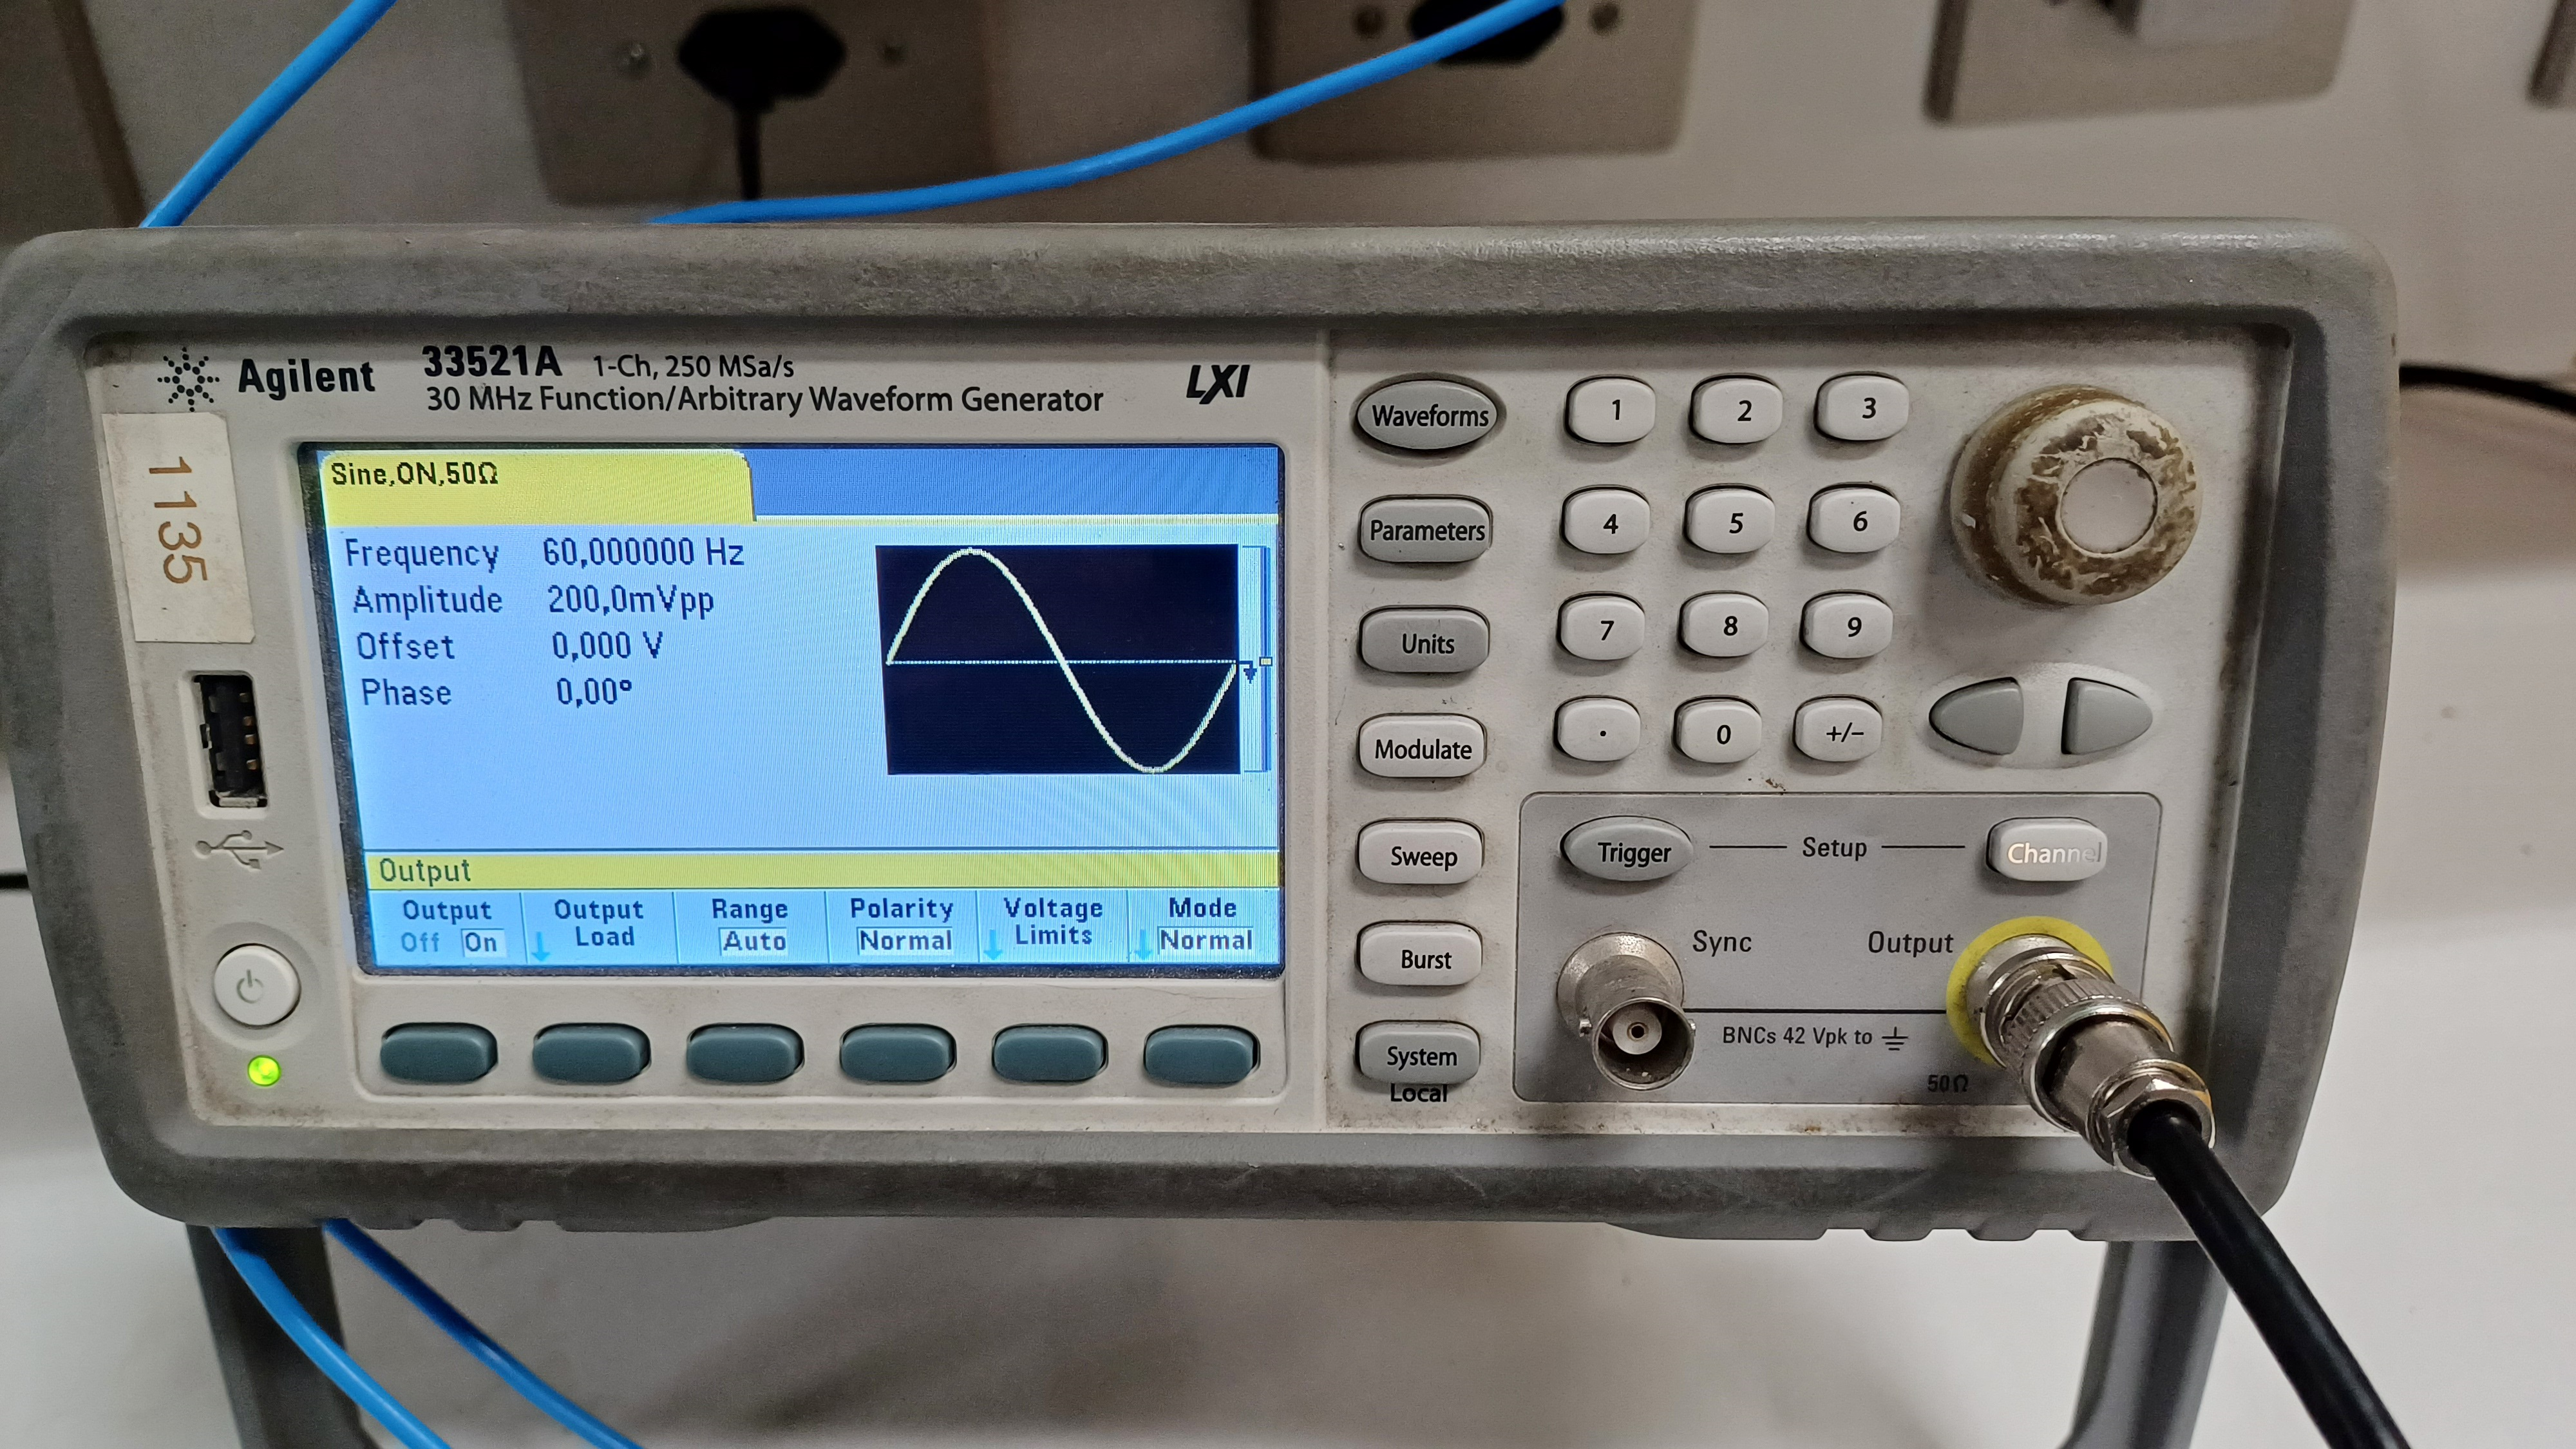
\includegraphics[width=0.8\textwidth]{figuras/ger-func-200.png}
    \fonte{}
\end{figure}

Utilizando-se novamente o osciloscópio e um multímetro, é possível comparar as leituras entre estes e o protótipo, respectivamente nas figuras \ref{fig:leitura-200-osc}, \ref{fig:leitura-200-mult}, \ref{fig:leitura-200-boy-onda} e \ref{fig:leitura-200-boy-valor}.

\begin{figure}[htb!]
    \caption{Leitura da onda de 200 mVpp - Osciloscópio}
    \label{fig:leitura-200-osc}
    \includegraphics[width=0.8\textwidth]{figuras/leitura-200-osc.png}
    \fonte{}
\end{figure}

\begin{figure}[htb!]
    \caption{Leitura da onda de 200 mVpp - Multímetro (valor RMS)}
    \label{fig:leitura-200-mult}
    \includegraphics[width=0.3\textwidth]{figuras/leitura-200-mult.png}
    \fonte{}
\end{figure}

\begin{figure}[htb!]
    \caption{Leitura da onda de 200 mVpp do protótipo - Onda}
    \label{fig:leitura-200-boy-onda}
    \includegraphics[width=0.8\textwidth]{figuras/leitura-200-boy-onda.png}
    \fonte{}
\end{figure}

\begin{figure}[htb!]
    \caption{Leitura da onda de 200 mVpp do protótipo - Valor}
    \label{fig:leitura-200-boy-valor}
    \includegraphics[width=0.8\textwidth]{figuras/leitura-200-boy-valor.png}
    \fonte{}
\end{figure}

Comparando os sinais obtidos, a diferença entre todos os diferentes instrumentos é notável neste range de leitura. O protótipo apresenta um erro fora do proposto pelas espeficicações. Este range pode ser melhor calibrado por software e seu erro curado a ponto de respeitar tais especificações. Nota-se também que existem valores de corrente e potências, porém o canal de tais não está conectado, sendo estes então descartáveis.

Finalmente, para a leitura de corrente na ordem de micro amperes, foi utilizado um resistor comum de 30 k$\Omega$, sendo este e seu valor representados pela \autoref{fig:res-30k}. Além disto, utilizou-se o gerador de função novamente para gerar uma tensão pequena de 10 Vpp ou 7.07 V. Com estes dados, utilizando novamente a lei de Ohm, se espera uma leitura de corrente de 0,000217 A ou 217 $\mu$A.

As leituras obtidas pelo multímetro e pelo protótipo são demonstradas respectivamente pelas figuras \ref{fig:leitura-micro-mult}, \ref{fig:leitura-micro-boy-onda} e \ref{fig:leitura-micro-boy-valor}.

\begin{figure}[htb!]
    \caption{Leitura da corrente de 217 $\mu$A - Multímetro.}
    \label{fig:leitura-micro-mult}
    \includegraphics[width=0.8\textwidth]{figuras/leitura-micro-mult.png}
    \fonte{}
\end{figure}

\begin{figure}[htb!]
    \caption{Leitura da corrente de 210 $\mu$A do protótipo - Onda.}
    \label{fig:leitura-micro-boy-onda}
    \includegraphics[width=0.8\textwidth]{figuras/leitura-micro-boy-onda.png}
    \fonte{}
\end{figure}

\begin{figure}[htb!]
    \caption{Leitura da corrente de 210 $\mu$A do protótipo - Valor.}
    \label{fig:leitura-micro-boy-valor}
    \includegraphics[width=0.8\textwidth]{figuras/leitura-micro-boy-valor.png}
    \fonte{}
\end{figure}

Olhando para os valores obtidos, percebe-se que o multímetro não apresenta um valor adequado, possívelmente por sua entrada de corrente no valor de micro estar queimada ou defeituosa. Já a leitura do protótipo está extremamente próxima do valor esperado, estando também dentro das especificações.

Finalmente, a tabela \ref{tab:resultados} contém todos os testes e seus resultados.

\begin{table}[!ht]
    \centering
    \caption{Resultados.}
    \label{tab:resultados}
    \begin{tabular}{|l|l|l|l|}
        \hline
        \textbf{Leitura} & \textbf{Osciloscópio} & \textbf{Multímetro} & \textbf{Protótipo}    \\ \hline
        Rede (V)         & 130 V                 & 128,7 V             & 128,1 V               \\ \hline
        Rede (A)         & -                     & 2,129 A             & 2,130 A               \\ \hline
        200 mVpp         & 143 mV RMS e 244 mVpp & 137 mV RMS          & 188 mV RMS e 263 mVpp \\ \hline
        217 $\mu$A       & -                     & 11,8 $\mu$A         & 210,7 $\mu$A          \\ \hline
    \end{tabular}
\end{table}
